\chapter{LITERATURE REVIEW}
\label{ch:litreview}

% \section{Introduction}

% This is a \LaTeX{} book~\parencite{urban1986introduction}.  \textcite{lamport1994latex} wrote a good~\LaTeX{} book. \textcite{Knu86book} claimed that \ldots

% \section{Previous Study on Problem B}

% Three or more authors \parencite{mittelbach2004latex}

% \textcite{mittelbach2004latex} has three or more authors.

% Two authors \parencite{kopka1995guide}.

% \textcite{kopka1995guide} has two authors.

% Cite more than one articles \parencite{urban1986introduction,lamport1994latex}.

% Newspaper \parencite{afp_covid_2021}.

% \section{Improved Method for Problem B}

% \lipsum[4-5]



\section{Dyslexia}

\subsection{Definition and Prevalence}

Dyslexia can be defined in so many ways. According to Merriam-Webster, dyslexia is defined as "a variable often familial learning disability involving difficulties in acquiring and processing language that is typically manifested by a lack of proficiency in reading, spelling, and writing" \parencite{mw:dyslexia}. The word's history dates back to 1888, where it is initially defined as an ``impairment in the ability to read due to a brain injury''. It is borrowed from French and German, where both it is written as \emph{dyslexie}. 

Estimates for the prevalence of dyslexia suggest that it affects around 5 to 17\% \parencite{Ramli2020} of the global population, marking it as one of the most common learning disorders. However, these statistics are subject to considerable variance due to the numerous definitions of dyslexia, the diverse methodologies employed for its diagnosis, and the sampling of different populations in research studies.

Despite these disparities in prevalence rates, what remains consistent is the universal recognition of dyslexia's significant impact on individuals' educational journeys, their professional progress, and even their day-to-day lives. It is also evident that dyslexia do not discriminate between genders alike, according to \textcite{Guerin1993DyslexicSA}.


\subsection{Causes and Risk Factors}
The causes of dyslexia are complex and multifaceted, involving an intricate interplay of genetic, neurobiological, and environmental factors. In fact, some of the causes are yet to be fully understood. 

Genetic researches have identified several genomic regions that have been linked to dyslexia, including chromosomes 6 and 18 \parencite{Francks2002, Schumacher2007}. Advancements in research has also found identifying candidate genes for dyslexia, which includes Dyslexia Susceptibility 1 Candidate Gene 1 (DYX1C1), Roundabout Guidance Receptor 1 (ROBO1), KIAA0319, and Doublecortin Domain Containing 2 (DCDC2) \parencite{Paracchini2007}. 

From a neurobiological standpoint, structural and functional differences have been identified in the brains of individuals with dyslexia. Neuroimaging studies have identified differences in brain structure and function in individuals with dyslexia, including disruptions in left hemisphere posterior brain systems and increased reliance on frontal lobe circuits \parencite{Kearns2019, Norton2015}.

Another research has found that dyslexia is highly heritable and displays polygenic transmission, and adult neuroimaging studies have found structural, functional, and physiological changes in the parieto-occipital and occipito-temporal regions, and in the inferior frontal gyrus, in adults with dyslexia \parencite{SorianoFerrer2017}. 

Another research also reviewed evidence of autopsy and structural imaging studies and found consistent evidence of symmetry of the planum temporale, thalamus, and cortical malformations in individuals with dyslexia \parencite{Wajuihian2011}.

Environmental factors further contribute to the manifestation and development of dyslexia. found that there is a substantial social-cultural bias in the delineation of literacy skills and in the definitions of reading disabilities, and suggests that phonological deficits should be emphasized as the core component in defining dyslexia \parencite{Samuelsson2003}.

\newpage
\subsection{Characteristics}
Dyslexia encompasses a variety of symptoms, which generally become apparent once a child starts school and is confronted with the challenges of learning to read and write. Common characteristics of dyslexia include difficulty with phonological skills, low accuracy and fluency of reading, poor spelling, and/or rapid visual-verbal responding \parencite{Roitsch2019}. 

These signs can vary in intensity and nature among individuals, contributing to the spectrum of dyslexia manifestations. Additionally, dyslexia can extend to erratic eye movements during reading and other tasks \parencite{Pavlidis1981}.

\subsection{Impact on Writing and Handwriting}
Dyslexia's impact extends noticeably to an individual's handwriting, with various studies indicating that individuals with dyslexia often grapple with handwriting fluency, neatness, and speed. A study found that children with dyslexia struggle with the graphomotor aspects of writing and are more impacted by the graphic complexity of words than typically developing children \parencite{Gosse2020}. 

Another study has also found that spelling ability influences the rate of handwriting production in children with dyslexia, and that productivity relies on spelling capabilities \parencite{Sumner2014}.

Writing speed also varies within children with dyslexia, as a study found that handwriting speed in Chinese children with dyslexia is related to deficits in rapid automatic naming, saccadic efficiency, and visual-motor integration \parencite{ChengLai2013}. 

Besides that, spelling deficits associated with dyslexia affect the dynamics of the interaction between central and peripheral processes and the level of anticipation that can be observed in word spelling in the context of a sentence to dictation task \parencite{SurezCoalla2020}.

\newpage
\subsection{Current Diagnostic Methods}
The diagnosis of dyslexia usually involves a holistic evaluation of the individual's academic performance, cognitive and linguistic skills, and developmental history. 

One study discusses the diagnostic assessment of dyslexia, which consists of standardized reading and spelling tests, evaluation of psychological state, and additional information from parents and teachers \parencite{SchulteKrne2010}. The diagnostic procedure may incorporate a battery of tests to assess reading, spelling, and writing skills. 

However, in recent times, studies have discovered advancements in diagnostic procedures. One research proposes a diagnostic method based on involuntary neurophysiological responses to auditory stimuli, using electroencephalogram signals to analyze temporal behavior and spectral content \parencite{Ortiz2020}. 

Another study has reviewed different technology-based approaches for dyslexia detection, including eye-tracking and Electroencephalogram (EEG) devices, and statistical or machine learning algorithms \parencite{Jankovic2022}.

\newpage
\subsection{Interventions and Treatments}
Even though there is no known cure for dyslexia, early assessment and intervention, paired with supportive teaching strategies, can significantly improve success rates for individuals with dyslexia. These interventions often include multi-sensory, structured language programs that explicitly teach phonics, morphology, syntax, and semantics. 

A study has found that multisensory, phonological, and cognitive training methods can be used to improve literacy and cognitive deficits among children with dyslexia in Malaysia \parencite{Anis2018}. 

Besides that, in Brazil, there are four key themes of interventions for dyslexia, which includes phonological-based intervention, computerized technology, auditory processing training, and visuomotor skills training \parencite{Signor2020}.

However, on a national level, governments have to make strides in dyslexia intervention. Study suggests that early identification of children at risk of dyslexia followed by evidence-based interventions is a realistic aim for practitioners and policy-makers 
\parencite{Snowling2012}. 

\newpage
\subsection{Challenges and Limitations of Current Practices}
Current practices in dyslexia diagnosis and intervention, despite their effectiveness, present several challenges. 

For one, the cognitive approach alone is not sufficient to address dyslexia, and that a combination of cognitive psychology, connectionism, and behaviorism is necessary \parencite{Tnnessen1999}.

A local study also finds that there is a lack of comprehensive studies that combine interventions for both cognitive functions and literacy deficits \parencite{Anis2018}. 

Besides that, while appropriate instruction can help at-risk readers become accurate and fluent, intensive remedial interventions have been less effective in closing the fluency gap. \parencite{Alexander2004}.


\newpage
\section{Machine Learning}
\subsection{Definition and Overview}
By definition, machine learning is the process by which a computer is able to improve its own performance by continuously incorporating new data into an existing statistical model. 

It can also be defined as "the branch of computer science dealing with the creation and use of computer software that employs machine learning" \parencite{mw:machine-learning}.

However, researchers have a differing opinion on the definition. One has defined machine learning as a branch of computational algorithms that emulate human intelligence by learning from the environment \parencite{ElNaqa2015}, while another describes machine learning as a study of computational methods for improving performance by mechanizing the acquisition of knowledge from experience \parencite{Langley1995}. 

Besides that, machine learning has also been described as a way to address problems where phenomena are changing rapidly, or where applications need to be customized for each user separately \parencite{Dietterich1996}.

Commonly, machine learning is classified into supervised, unsupervised, and reinforcement learning. However, there can also be semi-supervised, transduction and learning to learn algorithms \parencite{Oladipupo2010}. 

Supervised learning is typically used for prediction tasks, where a model is trained using labeled data meanwhile unsupervised learning involves finding hidden patterns or intrinsic structures from unlabeled data. Reinforcement learning enables a software agent to learn in an interactive environment by trial and error.

Within the broader machine learning landscape, a particularly noteworthy development is the emergence of deep learning. Deep learning is described as a network of nodes and edges that resemble the biological communication of brain neurons \parencite{Dinov2018}. 

Deep learning algorithms, often based on neural networks, can model high-level abstractions in data, thereby providing enhanced predictive accuracy in tasks such as image and speech recognition, natural language processing, and more.

\newpage
\subsection{Applications}
Machine learning's potential for pattern recognition and predictive analysis has led to a broad array of applications across multiple domains. This includes cyber security, healthcare, and intelligent transportation systems, to name a few. \parencite{Jhaveri2022}.

Socially, machine learning has made a big impact too. Social media has utilised machine learning to analyze large amounts of data, where for example Twitter, where it has been used to identify real and fake tweets \parencite{Arora2018}.

The reality is, machine learning is almost applied everywhere. A mobile phone is now capable of contextual search, object recognition, intelligent control, speech recognition, natural language processing, and computer vision, which is all powered by machine learning itself. As time goes on, the importance keeps getting even more significant as it slowly integrates to everyone's daily lives.

\newpage
\subsection{Machine Learning in Healthcare}
Healthcare stands out as a domain particularly poised to benefit from the advancements in machine learning. machine learning has been applied in a lot of areas, including medical imaging, natural language processing of medical documents, genetic information, disease prediction, disease detection, and personalized healthcare \parencite{Mana2022}.

Another key applications of ML in healthcare is in the field of medical imaging. In terms of radiology, it has shown that machine learning has potential to improve various aspects of radiology, including detection and interpretation of findings, postprocessing, and radiology reporting \parencite{Choy2018, Erickson2017}.

Another significant area of application is in predictive healthcare. machine learning algorithms Naïve Bayes, Decision Tree, Random Forest, and K-Nearest Neighbors are being utilised to predict diseases based on symptoms and large datasets of medical procedures \parencite{Garg2023}.

\newpage
\subsection{Feature Extraction and Selection}
Feature extraction and selection are crucial processes in any machine learning model. They involve identifying and selecting the most relevant information from raw data to be used for machine learning.

In the context of healthcare, feature extraction and selection could be applied to a variety of data, such as medical imaging, genomic data, or patient records. For instance, in Magnetic Resonance Imaging (MRI) feature extraction approach utilizes spatial filters, edge detection algorithms, and wavelet transform-based image fusion \parencite{Udomhunsakul}.

In handwriting analysis, features could refer to the stroke width, stroke length, speed, pressure, and slant among others. These characteristics can be critical in distinguishing between dyslexic and non-dyslexic handwriting. Selecting the right features is crucial as it directly impacts the performance of the machine learning model \parencite{Arif2015}.

\newpage
\subsection{Machine Learning Algorithms}
Machine learning algorithms are the crux of any machine learning model, determining how it learns from data and makes predictions or decisions. The choice of algorithm often depends on the nature of the task and the data at hand, with a wide range of algorithms available each with unique strengths and limitations.

Some of machine learning algorithms include K-Nearest Neighbors, Naïve Bayes, Support Vector Machine, Decision Tree, and others. These have been widely used in various fields, including healthcare, due to their interpretability and robustness \parencite{Ray2019}.

In recent years, deep learning algorithms, such as convolutional neural network and recurrent neural network, have gained popularity. These algorithms can learn complex patterns in data, making them highly effective for tasks that involve large amounts of data or that require the extraction of intricate features \parencite{Pamina2019SurveyOD}.

\newpage
\subsection{Performance Evaluation}
Evaluating the performance of machine learning models is essential to verify their effectiveness and reliability. Metrics such as accuracy, precision, recall, and F1 score are commonly used for this purpose. However, the choice of metrics should align with the problem at hand, as different tasks may require prioritizing different aspects of the model's performance.

In addition to these metrics, consideration of the model's robustness against variations in the data is crucial. This could involve testing the model under different conditions, or using different subsets of the data, to ensure that it performs consistently and does not overly rely on specific characteristics of the training data. 

There are a bunch of methods to evaluate robustness, including prediction consistency between source and target data in the neighborhood of the source samples \parencite{Shi2019} and a framework for evaluating robustness to changes in setting or population using a single, fixed evaluation dataset \parencite{Subbaswamy2020EvaluatingMR}.

Another important aspect of performance evaluation is the interpretability of the model. While some complex models, like deep learning models, may achieve high performance, they are often regarded as 'black boxes' due to their lack of interpretability \parencite{Zhang2018}. On the other hand, simpler models may offer more interpretability, but at the cost of performance. Striking a balance between these factors is an ongoing challenge in the field of machine learning.

\newpage
\subsection{Limitations and Challenges}
Despite the promising advancements, machine learning is not without its challenges and limitations. The quality and diversity of data is one of the primary concerns. machine learning models thrive on large amounts of high-quality, representative data. However, in situations where data is scarce, imbalanced, or inherently biased, the model's performance may be compromised \parencite{Lum2017}.

Another concern is overfitting, where the model learns the training data too well, to the point that it performs poorly on unseen data \parencite{Ying2019}. This issue highlights the importance of proper model validation and testing methodologies.

Data privacy is a crucial challenge across many domains that use machine learning. Ensuring the protection and appropriate use of sensitive data is a complex issue that often requires navigating regulatory and ethical considerations \parencite{Strobel2022}.

\newpage
\section{LeNet-5}
\begin{figure}[h]
    \centering
    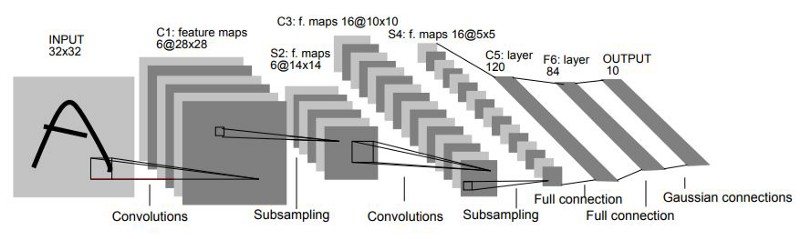
\includegraphics[scale=0.5]{mainmatter/images/literature review/lenet-5.jpeg}
    \caption{LeNet-5 architecture}
    \label{fig:LeNet-5}
    \textcite{Lecun1998}
\end{figure}

Le-Net 5 is a convolutional neural network (CNN) architecture proposed by \textcite{Lecun1998} for handwritten and machine-printed character recognition. It is a simple convolutional neural network and is widely used for image classification.

The neural network feautures a 7-level convolutional neural network. The input to the network is a 32x32 pixel image. The image is passed through the network and the output is a probability distribution over the 10 classes of digits (0-9). The architecture consists of two sets of convolutional and average pooling layers, followed by a flattening convolutional layer, then two fully-connected layers, and finally a softmax classifier \parencite{Lecun1998}.

LeNet-5 has been used in several researches, such as in \textcite{Isa2021CNNCM} and \textcite{isa2019automated}. 

% \newpage
% \section{Artificial Neural Network (ANN)}
% \begin{figure}[h]
%     \centering
%     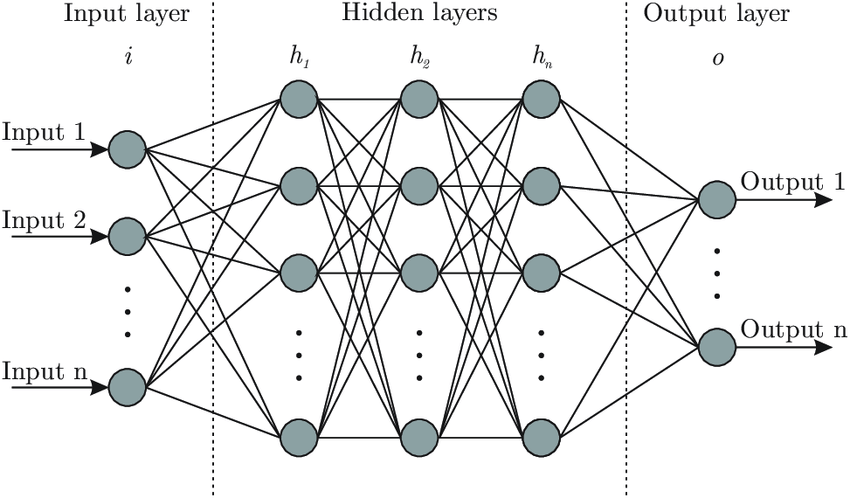
\includegraphics[scale=0.4]{mainmatter/images/literature review/ANN.png}
%     \caption{Artificial Neural Network architecture}
%     \label{fig:ANN}
%     \textcite{Bre2017}
% \end{figure}
% Artificial neural network (ANN) are a mathematical model that simulates the structure and functionalities of biological neural networks. ANNs are composed of interconnected processing elements (neurons) that work together to solve specific problems. ANNslearn by example and are configured for specific applications, such as pattern recognition or data classification, through a learning process. ANNs have the ability to extract patterns and detect trends that are too complex for humans or other computer techniques to notice \parencite{Krenker2011}.

% ANNs have remarkable ability to derive meaning from complicated or imprecise data, can be used to extract patterns and detect trends that are too complex to be noticed by either humans or other computer techniques \parencite{Zakaria2014ArtificialNN}.

% At the simplest level, an ANN consists of nodes (or 'neurons') connected by 'synapses', which transmit signals between the nodes. The strength of these connections, or weights, are adjusted during training, allowing the network to learn from the input data \parencite{Sonali2014ResearchPO}.

% ANNs have proven effective across a range of tasks, from image and speech recognition to natural language processing. One of their key strengths is their ability to learn and model non-linear and complex relationships, which makes them particularly useful in scenarios where the relationship between input and output is unknown or hard to define. 

% These applications include the use of ANNs in predicting properties of concrete-like composite materials \parencite{Kasperkiewicz2000}, to solve differential equations in radio frequency (RF) engineering \parencite{Pattanaik2008}, and in food science, including modeling microbial growth, interpreting spectroscopic data, and predicting physical, chemical, functional, and sensory properties of food products \parencite{Huang2007}. 

% However, despite its strengths, ANNs also have their challenges. One claims that it has two main limitations, which are over-training and its inability to extrapolate beyond the range of existing data \parencite{Yin2003}. Other than that, ANNs have difficulty of realizing non-linear sigmoidal activation functions \parencite{Mitra2016}.

% \newpage
% \section{Convolutional Neural Network (CNN)}
% \begin{figure}[h]
%     \centering
%     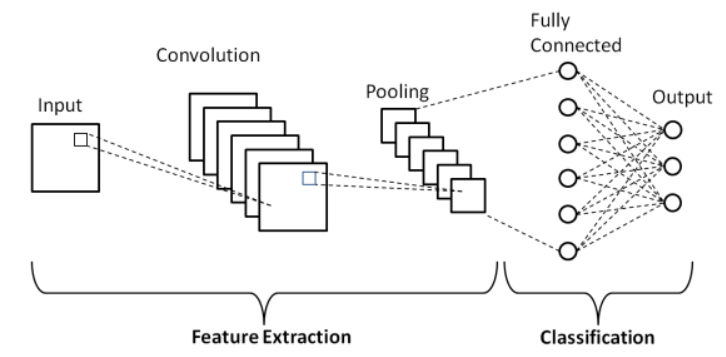
\includegraphics[scale=0.7]{mainmatter/images/literature review/CNN.png}
%     \caption{Convolutional Neural Network architecture}
%     \label{fig:CNN}
%     \textcite{Phung2019}
% \end{figure}
% Convolutional neural network (CNN) are a type of artificial neural network specifically designed for processing data with a grid-like topology, such as images. They have demonstrated impressive successes in applications such as computer vision for tasks such as face recognition, scene labeling, image classification, and natural language processing for speech recognition and text classification. \parencite{Bhandare2016ApplicationsOC} \parencite{TaiyabaAnsari2022}.

% The architecture of CNN is designed to mimic the way a human eye focuses on objects. It consists of one or more convolutional layers, often followed by pooling layers, fully connected layers, and normalization layers. The convolutional layer performs a convolution operation that focuses on small squares of input data, preserving spatial relationships between pixels \parencite{Purwono2023}.

% One distinctive feature of CNNs is the use of a technique known as 'weight sharing' in their convolutional layers, where the same filter (weights) is used for each part of the input. This allows the network to learn features that are useful across the entire image, reducing the number of parameters in the model, and thereby reducing overfitting.

% Despite their effectiveness, CNNs also have their challenges. They require substantial computational resources, making them expensive to train. Not just that, they lack true understanding and may make obvious mistakes, especially during deliberate testing rounds or on samples outside the training distributions \parencite{Yan2017HowIA}. 

% Furthermore, they require large amounts of labeled data, which may not always be available. CNNs are also susceptible to adversarial attacks, wherein small, purposely designed changes to input can lead the network to misclassify it.

% \newpage
% \section{Recurrent Neural Network (RNN)}
% \begin{figure}[h]
%     \centering
%     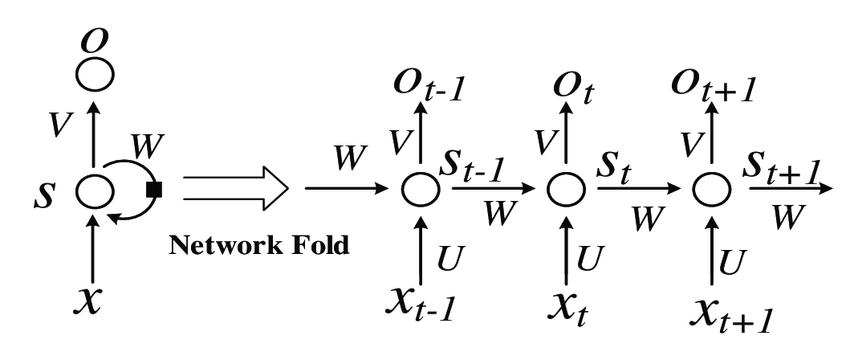
\includegraphics[scale=0.4]{mainmatter/images/literature review/RNN.png}
%     \caption{Recurrent Neural Network architecture}
%     \label{fig:ANN}
%     \textcite{Gao2018}
% \end{figure}
% Recurrent neural network (RNN) are a category of artificial neural network optimized for sequential data processing \parencite{Jain1999}. This makes them particularly suitable for tasks involving time-series data, such as speech recognition, natural language processing, or time series prediction.

% RNNs achieve their sequential data processing capability by incorporating loops within the network, allowing information to persist from one step in the sequence to the next. This 'memory' feature is what distinguishes RNNs from other neural network types, enabling them to effectively handle tasks that require understanding of context or the progression of inputs over time.

% One of the most common architectures of RNN is the Long Short-Term Memory network. LSTM overcome one of the key limitations of standard RNNs, which is the difficulty in learning long-range dependencies due to vanishing or exploding gradients \parencite{DiPietro2020}. By incorporating a gating mechanism, LSTMs can selectively remember or forget information, making them more efficient at processing sequences where context from much earlier steps is important.

% Despite their strengths, RNNs also present certain challenges. Training RNNs is difficult on 'chaotic' data as exploding and vanishing gradients keep occuring, which limits the expressivity of the RNN \parencite{Mikhaeil2021OnTD}. They can be computationally intensive and require careful optimization to prevent overfitting. Furthermore, while LSTMs address the vanishing gradient problem, they can still be complex to train effectively, and their inner workings can be hard to interpret.


\newpage
\section{Related Works}
\subsection{Existing Research}
Over the past few years, several research efforts have been dedicated to the application of machine learning for dyslexia. These studies have largely focused on aspects such as speech and language patterns, cognitive assessments, and reading behaviors.

However, the use of handwriting as a potential source of data for dyslexia detection has been less explored. Early efforts have indicated the promise of this approach, leveraging machine learning techniques to identify unique features in dyslexic handwriting and assess their correlation with dyslexia.

Despite the potential, much of the existing research is in its early stages, and many studies have been conducted on a small scale or under controlled conditions. Thus, while the preliminary results are encouraging, there is still much to understand about the effectiveness of these techniques when applied to more diverse and larger-scale real-world contexts.

This emerging field presents an opportunity for new research to contribute to both the understanding of dyslexia through handwriting analysis and the development of effective machine learning techniques for dyslexic handwriting detection.

\newpage
\subsection{Data Used in Previous Studies}
Previous studies investigating dyslexic handwriting detection with machine learning have made use of various types of data. In many cases, these include handwriting samples collected from both dyslexic and non-dyslexic individuals, often children.

Handwriting samples can come in various forms, such as isolated characters, words, or continuous texts. Each of these forms provides different levels of complexity and contextual information, which could influence the detection performance.

In addition to the handwriting samples themselves, some studies also utilize supplementary data, such as demographic information, educational history, and details of dyslexia severity or related symptoms. This additional information could help in contextualizing the handwriting features and improving the prediction models.

The choice of data, its collection, and pre-processing significantly impact the results of the machine learning models. Therefore, understanding the types and characteristics of data used in existing studies can provide valuable insights for future research.

Furthermore, some datasets, such as \textcite{Isa2021CNNCM}, made their datasets publically available through Kaggle, a data science platform and online community of data scientists and machine learning practitioners made by Google.

\newpage
\subsection{Feature Extraction in Handwriting Analysis}
Feature extraction plays a crucial role in the analysis of handwriting for dyslexia detection. This process involves identifying and quantifying characteristics in the handwriting samples that could potentially differentiate between dyslexic and non-dyslexic individuals.

Features extracted from handwriting can be categorized into static and dynamic features. Static features are derived from the visual appearance of the written text and include aspects such as letter shape, size, slant, and spacing. 

On the other hand, dynamic features capture the process of writing and may include pen pressure, velocity, and acceleration, among others. In \parencite{Lam2011ChineseHP}, the pressure of the pen was captured using the Wacom digitizer, allowing for more in-depth data regarding the handwriting.

Machine learning methods, particularly deep learning, have also been used to automatically extract features from handwriting samples. These techniques can learn to identify complex patterns in the data without the need for manual feature engineering, potentially uncovering novel features of dyslexic handwriting. 

\textcite{Isa2021CNNCM} has used the convolutional layer work as the feature extractor where the layer studies the feature representations of input images. Then, the trainable convolutional kernel will regulate its kernel weights automatically in backpropagation training process.

However, the choice of features and extraction methods can significantly influence the performance of dyslexic handwriting detection. Hence, understanding the approaches used in previous studies can help guide the selection and development of feature extraction techniques in future research.


\newpage
\subsection{Techniques, Performance and Findings}
Various machine learning techniques have been employed in previous studies to analyze handwriting for dyslexia detection. These range from traditional machine learning methods to more recent deep learning models.

Deep learning models, including artificial neural network and convolutional neural network, have also been applied to this task. artificial neural networks, in this context has been used in \textcite{isa2019automated}. In contrast, convolutional neural networks are utilised in \textcite{Isa2021CNNCM}, in the form of LeNet-5.

Each of these techniques has its strengths and limitations and may be more or less suitable depending on the specific characteristics of the data and task. Therefore, a thorough understanding of the machine learning techniques used in existing studies is crucial for informing the choice of methods in future research.

The performance of machine learning techniques in detecting dyslexic handwriting varies widely across different studies, largely due to the differences in data used, features extracted, and the specific models applied.

Many of these studies report varying results. These findings suggest that machine learning has potential in identifying dyslexic handwriting and could aid in early and more accurate diagnosis.

In \textcite{Isa2019AutomatedDO}, the accuracy of the ANN model is reported to be at 73.33 percent. Later in 2021, having switched to the CNN model, \textcite{Isa2021CNNCM} has reported training accuracies as high as 0.985 on the CNN-1 model, while other models received slightly lower accuracies of 0.98 and 0.968. 

On the other hand, through the random forest approach, \textcite{Richard2020DyslexiaAD} has achieved 90 percent accuracy using the model. However, not all studies has achieved high accuracy. 

A study from \textcite{Drotr2020DysgraphiaDT} has obtained only a 79.5 percent prediction accuracy using the AdaBoost algorithm. Furthermore, \textcite{Spoon2019TowardsDD} has reported an accuracy of only 55.7 percent in its research.

It is also important to note that many of the reported studies have been conducted under controlled conditions and on small, often homogeneous datasets. Therefore, it remains to be seen whether these results can be generalized to more diverse and larger populations.

Considering the current state of research, while the initial results are encouraging, there is still much work needed to validate and refine these techniques for practical use. More comprehensive studies, involving larger and more diverse samples, are required to establish the reliability and applicability of these techniques.

\newpage
\subsection{Challenges and Limitations}
While the use of machine learning for dyslexic handwriting detection presents exciting opportunities, it also comes with several challenges and limitations that have been identified in previous research.

One of the major challenges lies in the data itself. Handwriting can vary widely between individuals and can be influenced by numerous factors such as age, education, and cultural background. This variability makes it challenging to develop models that are generalizable across diverse populations.

Additionally, even though getting data sets are getting easier day by day, especially through open platforms, such as Kaggle, obtaining large quantities of labeled handwriting data from dyslexic individuals for training machine learning models can be difficult due to privacy concerns and the excruciatingly time-consuming nature of data collection and labeling.

From a technical perspective, the choice of features and machine learning algorithms can significantly impact the performance of the models. Yet, there is still currently no consensus at all on the optimal features or models for dyslexic handwriting detection, making it a challenging area of research.

Furthermore, while deep learning methods have shown promise in this field, they come with their own set of challenges. They typically require large amounts of data, significant computational resources, and often times their complex models are severely lacking in interpretability, which is crucial in healthcare applications.

Despite these challenges, all of the researches done so far has laid a solid foundation for future work in this area. By understanding and addressing these limitations, future research can contribute to the development of more effective and practical solutions for dyslexic handwriting detection.

\newpage
\subsection{Future Directions and Opportunities}
As the research in dyslexic handwriting detection using machine learning continues to evolve, several promising directions and opportunities have been identified.

One such direction is the further exploration of deep learning techniques. Despite the challenges, their potential in automatically extracting complex features from handwriting samples and handling large-scale datasets make them a promising area for future research. There were also suggestions of trying out unsupervised approaches, which includes clustering to group the data into clusters that could then be inspected by human experts \parencite{Spoon2019TowardsDD}.

Moreover, more comprehensive and diverse datasets can vastly enhance the generalizability and reliability of the models. Efforts to create larger, more diverse datasets that encompass a range of handwriting styles, demographic backgrounds, and dyslexia severities are needed. This claim has been generally voiced by many studies, that includes studies from \textcite{Isa2019AutomatedDO}, \textcite{Richard2020DyslexiaAD} and \textcite{Usman2021AdvanceML}.

Lastly, more research into the interpretability of machine learning models can also be valuable. Developing models that not only perform well, but also provide insights into their decision-making process can enhance trust and adoption of these techniques in real-world settings.

In conclusion, while the field of dyslexic handwriting detection using machine learning is still in its early stages, the initial findings are promising and point towards a future with more accurate, timely, and accessible dyslexia detection tools.\\

\newpage
\section{Summary}
To summarise everything in Literature Review, this study reviews dyslexia and its impact on handwriting. Besides that, this study discovers machine learning and its use in dyslexic handwriting detection, where then a machine learning model, which is LeNet-5, is used to perform dyslexic handwriting detection. 

A comprehensive review of previously done researches relevant to dyslexic handwriting detection using machine learning has been done. Finally, the spirit of research itself, there will definitely always be new discoveries to be found in the study. 